% Explore the strategy of varying dialect by observing openvpn
% (1) tightening constraint on edge can remove unwanted or vulnerable component
% (2) preserving constraint on edge can also cause the change to outfacing interface
% (3) relaxing constraint is not a good idea because (1) introducing non-deterministic (2) enlarge attack surface
% (4) Add new states
% (5) Remove states through message removal
% (6) Add State though introducing new messages

\newpage

\section{Generating Various Dialects}
\label{sec:dialect}

With finite state machines extracted, we now discuss how we plan to customize a
protocol implementation to generate various dialects. To be specific, we first
discuss the challenges of protocol dialect generation. Then, we discuss how we
plan to tackle these challenges.

\subsection{Challenges}
\label{sec:task2:challenges}

Dialect generation needs to take as input a protocol implementation, and
generate various dialects. To achieve this, we have to address two major
challenges below.

\begin{wrapfigure}{r}{0.4\textwidth}
  \centering
  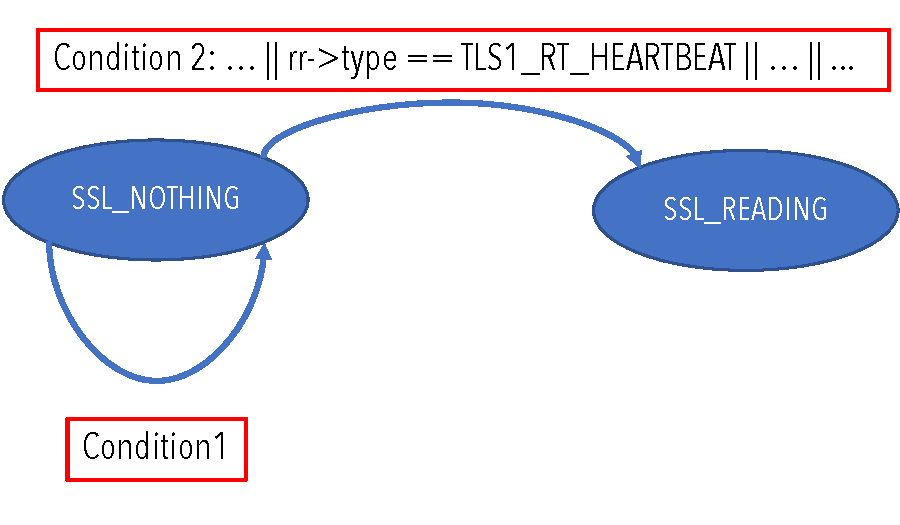
\includegraphics[width=0.4\textwidth]{figure/constraint_tighten}
  \caption{A state machine manually extracted from \texttt{OpenSSL}.}
  \label{fig:tighten}
\end{wrapfigure}

\noindent{\textbf{Recovering protocol dialects.}} The prerequisite for dialect
generation is to recover the original dialect from a protocol implementation.
To do this, an instinctive reaction is to use static analysis techniques to
identify the messages exchanging between parties. However, the research in the
past mostly focuses on performing static analysis on a single code base, and
software developers typically implement communication protocols in multiple
code bases and even involving multiple parties. As a result, our first
technical challenge for dialect generation is to design an effective approach
to restore dialects from protocol implementation.

\noindent{\textbf{Ensuring protocol validity.}}  Even though we are able to
recover dialects encoded in source code, dialect generation is still
challenging. To generate a new dialect, there are many possible strategies.
However, many of them may not guarantee the reliability (or validity) of a
dialect newly generated (\eg, generating a new dialect for \texttt{TCP}
communication by eliminating the three-way handshake). As a result, the second
challenge of dialect generation is to identify a set of effective strategies
that can generate new protocol dialects but not introduce incorrectness.

\subsection{Proposed Techniques}

In the following, we propose a series of techniques to address the challenges above. More specifically, we first introduce how we plan to recover protocol dialects using the state machines extracted. Then, we discuss how we intend to generate new valid dialects by varying state machines. 

\subsubsection{Research Task 4: Recovering Protocol Dialects}

In the context of protocol customization, it is generally challenging to achieve a clean code removal. Take the condition tightening strategy for example. As is illustrated in Figure~\ref{} and~\ref{}, we can easily pinpoint the code fragment corresponding to the removal condition. However, this is far from sufficient for clearly cutting off the code unnecessary for protocol dialects newly generated. As is mentioned in Section~\ref{sec:task2:challenges}, a communication protocol typically involves multiple parties, and a software developer may implement a protocol across different code bases and even through multiple threads. To perform a clean code removal, we must design and develop a mechanism to link all the code fragments to the one directly presented under the removal condition.  

In this project, we plan to enable this mechanism by recovering protocol dialects from implementations using the following approaches. To be specific, we will first identify the finite state machines that involve communication dialects. Since a communication dialect involves message exchanging, we intend to achieve this by examining state machines tied to function calls responsible for message sending and receiving. Second, we will pair state machines tied to the same dialect. To accomplish this, we plan to examine the data structure tied to function calls. Here, our hypothesis is that, if sending and receiving function calls are all tied to the same data structure, the corresponding state machines are involved to the same dialect. In this project, we will validate this hypothesis and if needed adjust this technique based on protocol implementations. 

After identifying and pairing state machines, we will then recover the sequence of the messages exchanged between the paired state machines. To do this, we plan to  perform value set analysis on the code base corresponding to each of the state machines. Similar to the technique proposed for refining a state machine in Section~\ref{}, we will conduct this analysis against the outgoing messages prior to its attachment to message sending, and then match that value set with transition conditions of the state machine present on the other side. To illustrate this approach, we take \texttt{OpenVPN} for example. By performing a value set analysis at the site where a client state machine sends a request message, we obtain a set of values for the message which perfectly match transition condition \Code{!(&ks->plaintext_write_buf->len) && !session->opt->server && packet.opcode == P_CONTROL_HARD_RESET_CLIENT_V2} present on the edge of a server state machine.   


With protocol dialect restored, it is not difficult to notice that one could easily pinpoint the messages exchanged between each other which can be further used for tracking down the code fragments pertaining to that of removal. For example, by tightening the condition on transition from state \texttt{S\_PRE\_START} to \texttt{S\_START} illustrated in Figure~\ref{fig:original_dialect}, we can use the dialect to pinpoint the call to that function responsible for sending \texttt{P\_ACK}. On the code base running on the client side, we can then perform backward taint and identify the code fragments relevant to message \texttt{P\_ACK} holding the removed condition. In this project, we will use the output of this backward taint to guide our code fragment removal.

\subsubsection{Research Task 5: Customizing Dialect with Transition State Variation}

\begin{wrapfigure}{r}{0.4\textwidth}
  \centering
  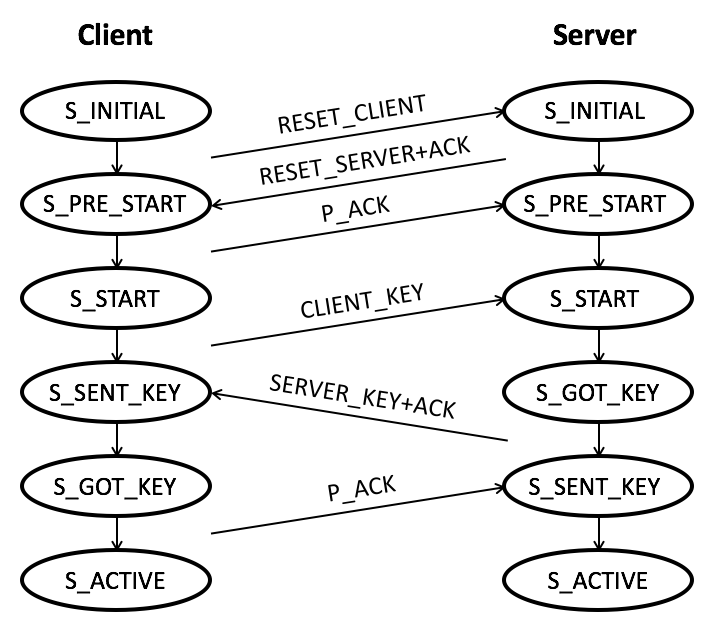
\includegraphics[width=0.4\textwidth]{figure/openvpn_protocol}
  \caption{The protocol dialects implemented in \texttt{OpenVPN} responsible for establishing a private communication tunnel. Note that the ovals indicate transition states in finite state machines extracted from a target protocol, and the edges between them demonstrate the transitions from on state to another.}
  \label{fig:original_dialect}
\end{wrapfigure}

To tackle the second challenge mentioned above, we propose two strategies to mutate transition states and thus vary dialects. In this project, we plan to develop the techniques involved and validate each of these strategies with more applications.    

{\noindent{\textbf{Eliminating states with message merging}} is our first strategy where we preserve protocol semantic by removing a state and merging the message eliminated with a consecutive message. To illustrate this, we take \texttt{OpenVPN} for example. As is shown in Figure~\ref{fig:detleted_dialect}, we first trim transition state \texttt{S\_PRE\_START} and disable the function responsible for sending message \texttt{P\_ACK}. Second, we change the target state under condition \texttt{C1} and append the information carried by \texttt{P\_ACK} to consecutive message \texttt{CLIENT\_KEY}. To be able to check message \texttt{P\_ACK} piggybacking on \texttt{CLIENT\_KEY}, we finally concatenate the transition conditions with a logic conjunction operator. In this way, we preserve the message needed for the 3-way handshake in a consecutive message. Thus, it guarantees the legitimacy of the new dialect. In this project, we will take this state elimination as \emph{the third strategy} for our dialect generation.

{\noindent{\textbf{Introducing states with message partition}} is a strategy in which we introduce not only new states but also partition messages. Again, we take \texttt{OpenVPN} for example. As is illustrated in Figure~\ref{}, on the client side, we first insert additional state \texttt{EXTRA\_CLIENT} between states \texttt{S\_PRE\_START} and \texttt{S\_START} by changing the target state under condition \texttt{C2'}. Second, we partition condition \texttt{C2'} into two individual constraints \texttt{C2.1'} and \texttt{C2.2'} so that the disjunction of these two is equivalent to \texttt{C2'} (\ie, \Code{C2.1' || C2.2' = C2'}). Third, we replace transition condition \texttt{C2'} with \texttt{C2.1'}, and introduce a new transition from state \texttt{S\_EXTRA} to state \texttt{S\_START} under condition \texttt{C2.2'}. 

Since condition \texttt{C2.1'} is the tightened version of \texttt{C2'}, and message \texttt{RESET\_SERVER+ACK} is not able to trigger the state transition from \texttt{S\_PRE\_START} to \texttt{S\_EXTRA}, we could perform a backward taint analysis from the site where the server sends message \texttt{RESET\_SERVER+ACK}. The goal of this backward taint analysis is to identify the code fragments relevant to the outgoing message \texttt{RESET\_SERVER+ACK}. With this, we will adjust the implementation based on the condition replaced, and synthesize a code snippet capable of generating a message that can trigger the transition from state \texttt{S\_EXTRA} to state \texttt{S\_START
}. In this project, we will insert this code snippet on the server into the implementation indicating the transition from state \texttt{S\_PRE\_START} to state \texttt{S\_START}. 

\subsubsection{Research Task 6: Customizing Dialect with Transition Condition Variation}

% To generate new valid dialects, we will first explore how to generate new valid dialects by varying state transitions. To be specific, 

Since a protocol dialect typically relies upon finite state machines, our study first focuses on exploring how to generate new valid dialects by varying state transitions. To be specific, we manually studied three strategies to vary transition conditions. 


\begin{wraptable}{r}{.38\textwidth}
\centering
\begin{tabular}{c}
\hspace{12pt}

\begin{lstlisting}  
else if (rr->type == TLS1_RT_HEARTBEAT) {
  dtls1_process_heartbeat(s); /* Vulnerable function */
  rr->length = 0;
  s->rwstate=SSL_READING;
  BIO_clear_retry_flags(SSL_get_rbio(s));
  BIO_set_retry_read(SSL_get_rbio(s));
  return(-1);
}
\end{lstlisting}

\end{tabular}
\caption{A code snippet under the condition eliminated vulnerable to the heartbleed bug.}
\label{code:heartbleed}
\end{wraptable} 

\noindent{\textbf{Tightening transition conditions}} is a strategy where we eliminate some conditions to tighten the constraint of triggering a state transition. To illustrate this, we take for example the state machine manually extracted from \texttt{OpenSSL} (see Figure~\ref{fig:tighten}). By removing condition \Code{rr->type == TLS1_RT_HEARTBEAT} on the state machine as well as the corresponding implementation in source code, we could tighten the condition pertaining to the transition from state \texttt{SSL\_NOTHING} to \texttt{SSL\_READING}, and cut off the heartbeat component vulnerable to the heartbleed bug~\citep{} (see Table~\ref{code:heartbleed}). Since the heartbeat component is optional for \texttt{OpenSSL}, we could obtain a new valid dialect without the heartbeat messages exchanged between a client and a server. In this project, we will take this condition tightening as \emph{the first strategy} for generating new dialects. 

\begin{wrapfigure}{r}{0.4\textwidth}
  \centering
  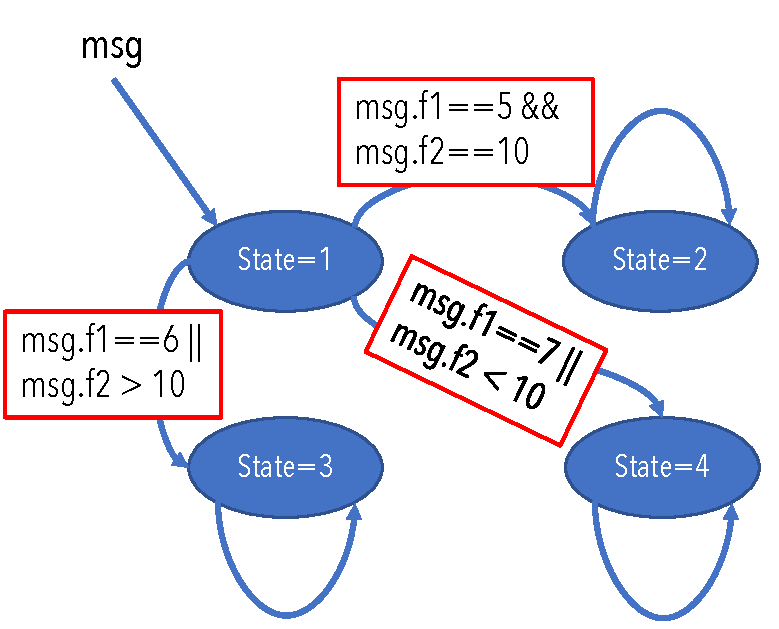
\includegraphics[width=0.4\textwidth]{figure/toy}
  \caption{A toy state machine taking as input message \texttt{msg} from a client side. Note that the constraints in the text boxes indicate transition conditions, and the message carries integer data in two fields -- \texttt{msg.f1} and \texttt{msg.f2}.}
  \label{fig:toy_fsm}
\end{wrapfigure}

\noindent{\textbf{Relaxing transition conditions}} is another strategy, in which we get rid of a condition to relax the constraint of triggering a state transition. To illustrate this, we take for example a toy protocol, a finite state machine of which is shown in Figure~\ref{fig:toy_fsm}. By getting rid of condition \Code{msg.f2==10}, we can relax the constraint pertaining to the transition from state \texttt{1} to state \texttt{2}. It is not difficult to note that such a mutation practice introduces non-deterministic to the state machine newly generated, especially when the input message holds condition \Code{msg.f1==5 && msg.f2 > 10}. As a result, we believe this transition mutation is not suitable for generating a new dialect. In this project, we will avoid performing dialect generation by following this strategy.

\begin{figure*}
  \centering
  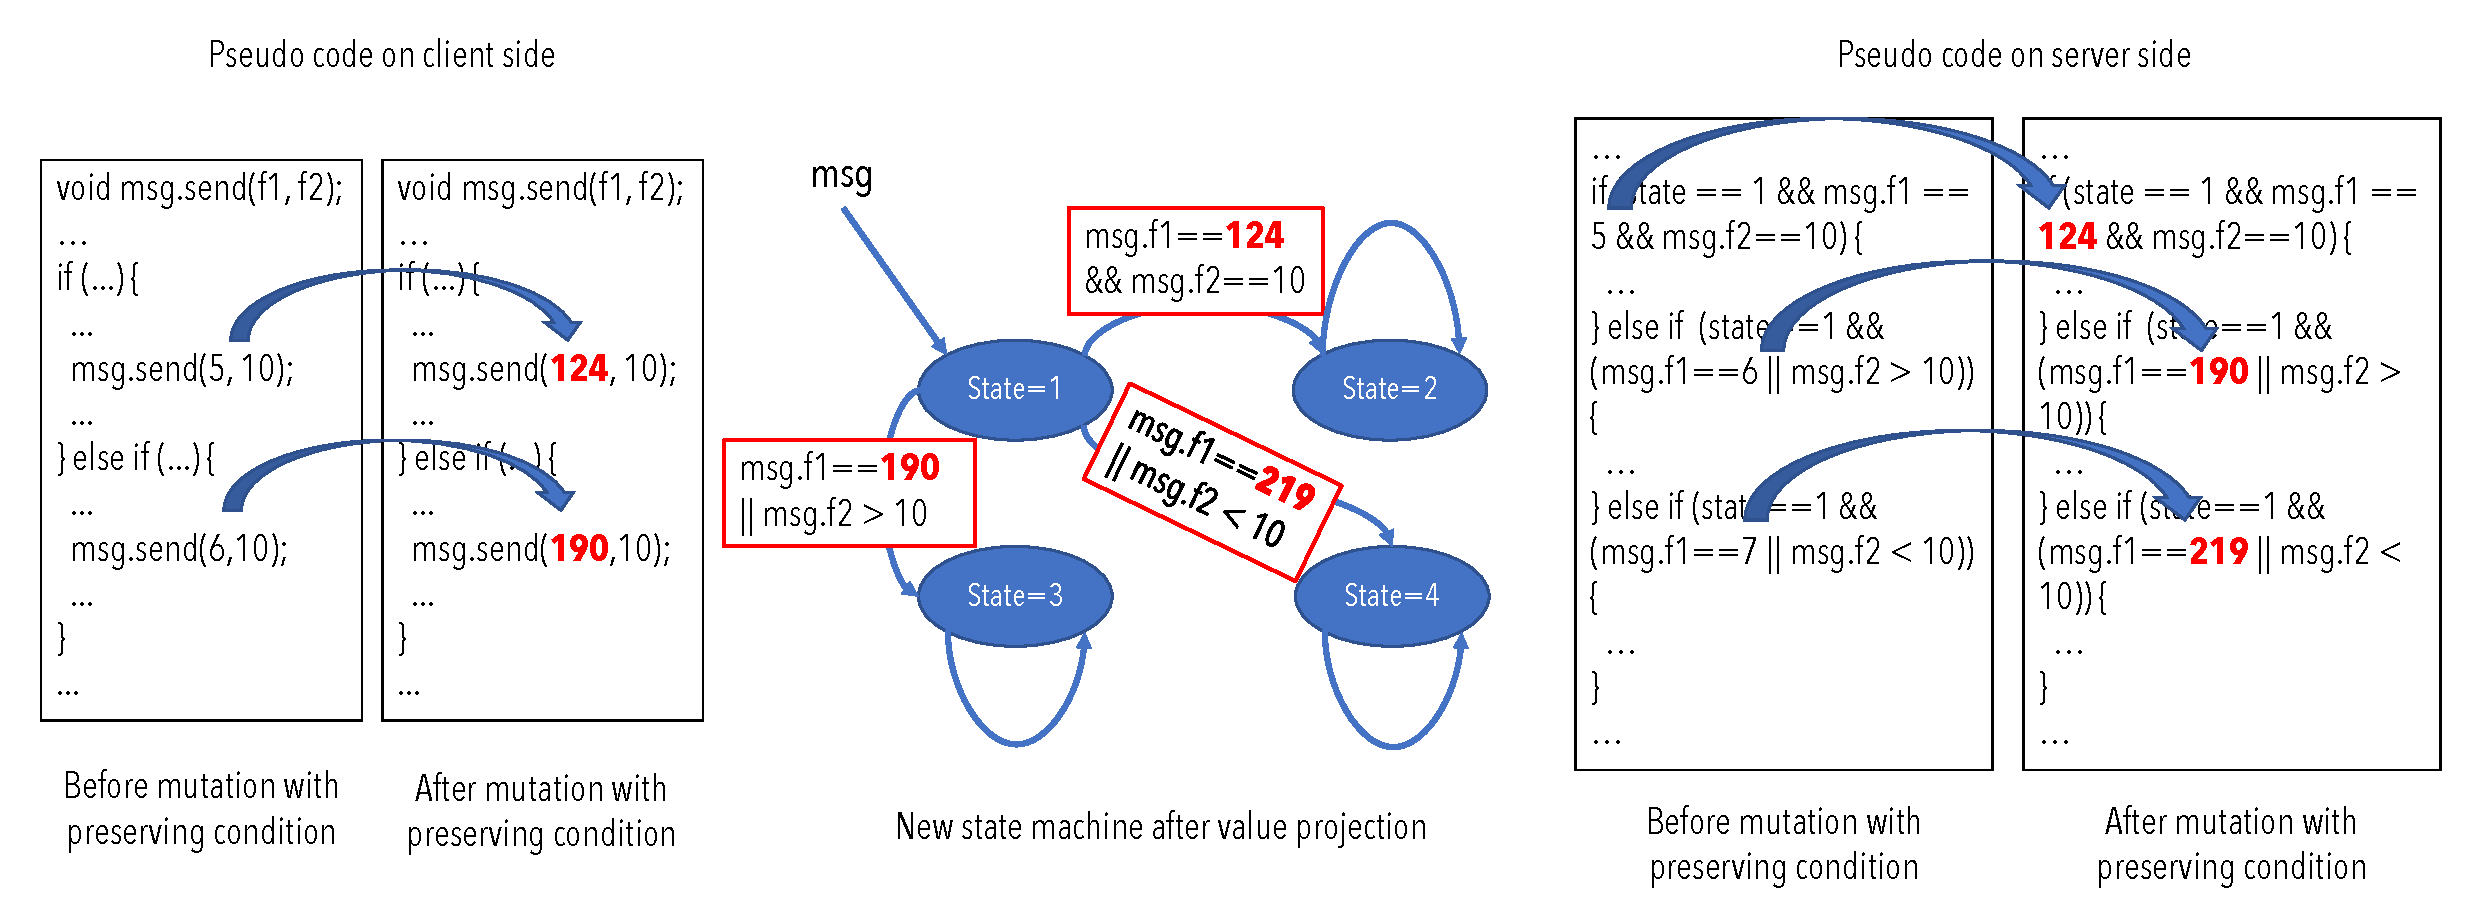
\includegraphics[width=0.95\textwidth]{figure/shuffle}
  \caption{The new state machine and pseudo code generated by following the strategy of preserving transition conditions.}
  \label{fig:toy_shuffle}
\end{figure*}

\noindent{\textbf{Preserving transition conditions}} is a strategy where we vary individual transition conditions and at the same time preserve the one indicating their combination. To illustrate this, we again take for example the state machine shown in Figure~\ref{fig:toy_fsm}. Assume \texttt{msg.f1} in condition \Code{msg.f1==5 && msg.f2==10} is an integer variable with the values from 5 to 7, indicating the operation code received from a client side. By shuffling these three values on the state machine and modifying the corresponding implementation on both ends (see Figure~\ref{fig:toy_shuffle}), we can change the state machine to a new one -- with the only difference in the state transitions -- and thus generate a new dialect in which both the client and server use new messages to coordinate the state transition. In this project, we will take this as \emph{the second strategy} for customizing protocol dialects. 





























































% \begin{figure*}[t]
% \centering
% \subfloat[Original Dialect.]{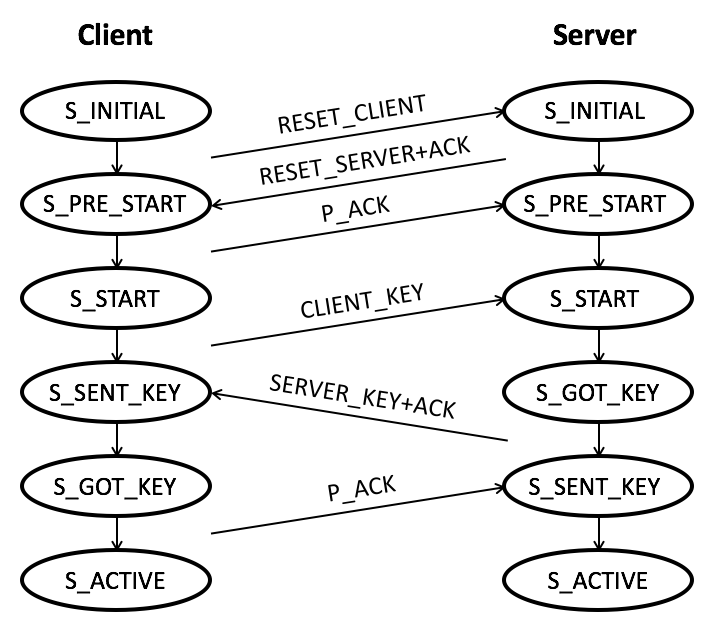
\includegraphics[width=0.33\linewidth]{figure/openvpn_protocol}\label{fig:original_dialect}} 
% \subfloat[Dialect with state removal.]{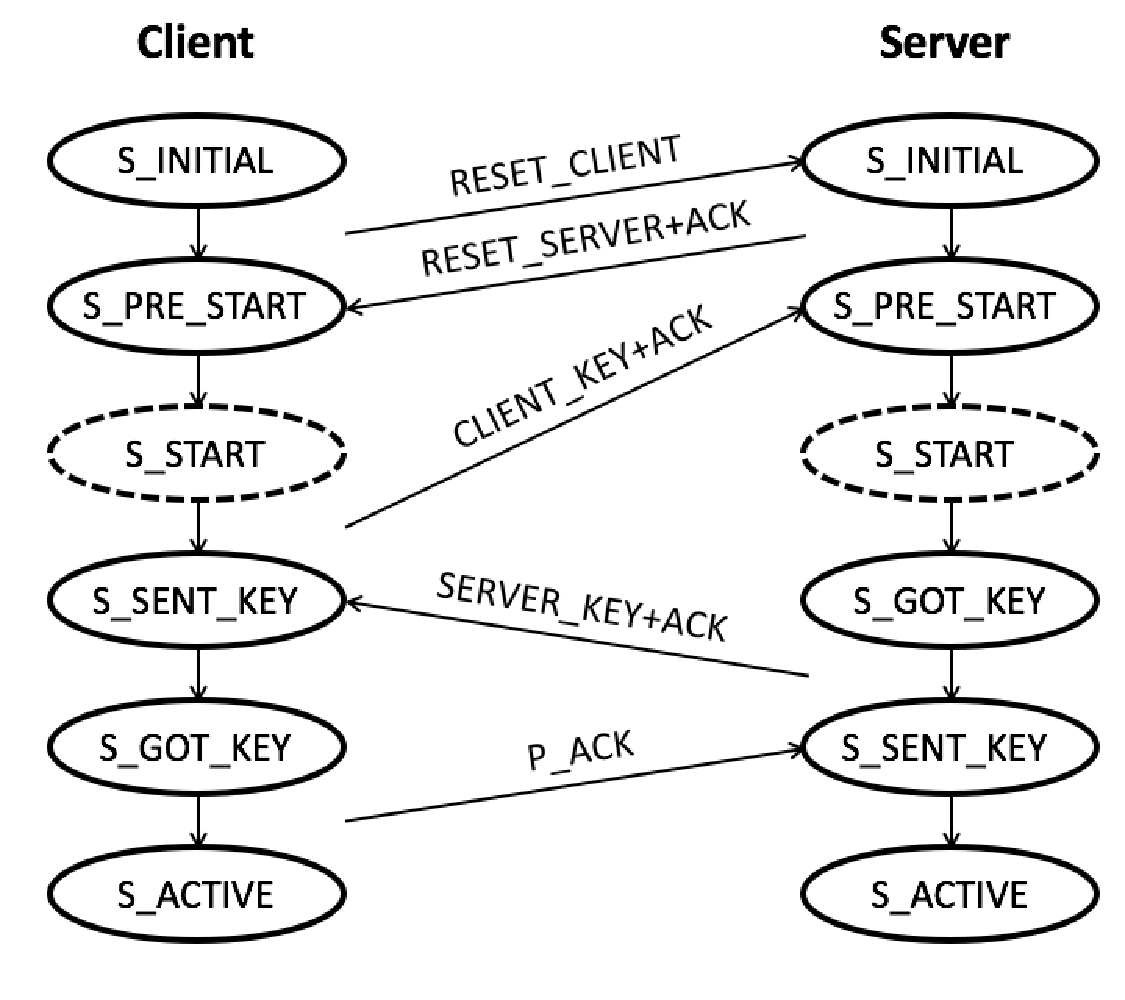
\includegraphics[width=0.33\linewidth]{figure/mutation4}\label{fig:detleted_dialect}}
% \subfloat[Dialect with state addition.]{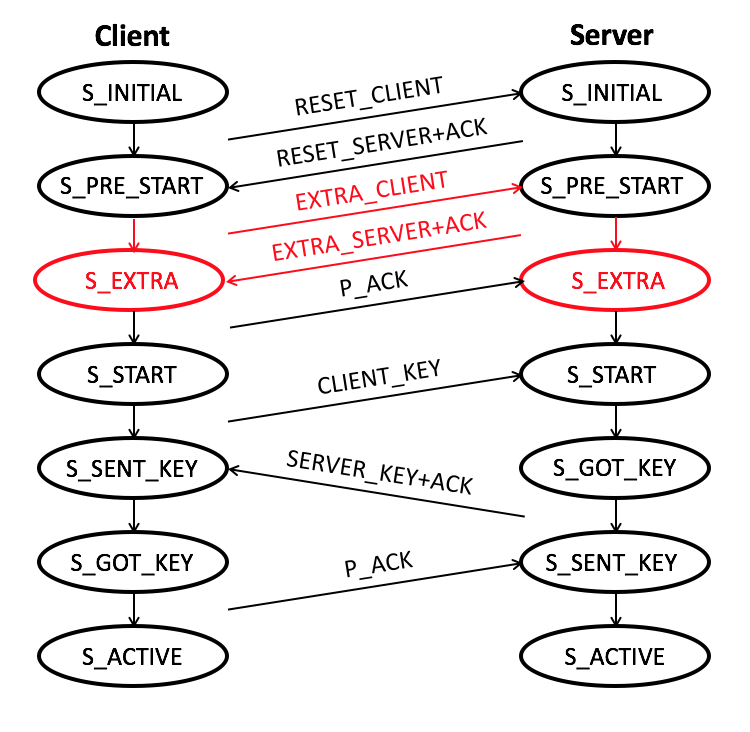
\includegraphics[width=0.33\linewidth]{figure/mutation3}\label{fig:added_dialect}} 
% \vspace{-0.1in}
% \caption{The protocol dialects implemented in \texttt{OpenVPN} responsible for establishing a private communication tunnel. Note that the ovals indicate transition states in finite state machines extracted from a target protocol, and the edges between them demonstrate the transitions from on state to another.} 
% \label{fig:dialect} 
% \end{figure*} 








